\documentclass[12pt,a4paper]{report}
% ============================================================================
%  RAJALAKSHMI ENGINEERING COLLEGE - MINI PROJECT / RESEARCH REPORT
%  Verify-or-Reject Grounding (VoRG)
%  House style adapted from the FundTrail internship report.
% ============================================================================
\usepackage[a4paper,top=2.5cm,bottom=2.5cm,left=3cm,right=2.5cm]{geometry}
\usepackage[T1]{fontenc}
\usepackage{newtxtext,newtxmath}
\newcommand{\Usefont}[1]{\fontfamily{#1}\selectfont}
\usepackage{graphicx}
\usepackage{setspace}
\usepackage{array}
\usepackage{booktabs}
\usepackage{tabularx}
\usepackage{enumitem}
\usepackage{titlesec}
\usepackage{titletoc}
\usepackage{fancyhdr}
\usepackage{xcolor}
\usepackage{colortbl}
\usepackage{amsmath}
\usepackage{algorithm}
\usepackage{algpseudocode}
\usepackage{tikz}
\usetikzlibrary{arrows.meta,positioning,fit,backgrounds,shapes.geometric,calc}
\usepackage{float}
\usepackage{caption}
\usepackage{microtype}
\usepackage{indentfirst}
\usepackage{mdframed}
\usepackage[hidelinks]{hyperref}

\setlength{\headheight}{16.14995pt}
\addtolength{\topmargin}{-4.14995pt}

\definecolor{navy}{RGB}{0,0,0}
\definecolor{navysoft}{RGB}{60,60,60}
\definecolor{steel}{RGB}{95,95,95}
\definecolor{rulegray}{RGB}{150,150,150}
\definecolor{rowgray}{RGB}{240,240,240}
\definecolor{rowblue}{RGB}{232,232,232}
\definecolor{accentline}{RGB}{80,80,80}
\definecolor{okgreen}{RGB}{60,110,60}
\definecolor{warnred}{RGB}{150,50,50}

\onehalfspacing
\setlength{\parindent}{1.5em}
\setlist{itemsep=2pt,parsep=0pt,topsep=4pt,leftmargin=1.6em}
\captionsetup{font=small,labelfont={bf,color=navy},labelsep=period}
\captionsetup[figure]{name=Fig.}
\captionsetup[table]{name=Table}

% ---- Plain numbered chapter heading: "1  INTRODUCTION", no "Chapter" word ----
\titleformat{\chapter}
  {\normalfont\huge\bfseries\color{navy}\filright}
  {\thechapter}
  {1em}
  {\MakeUppercase}
  [\vspace{4pt}{\color{accentline}\titlerule[2pt]}\vspace{-5pt}{\color{navy}\titlerule[0.6pt]}]
\titlespacing*{\chapter}{0pt}{8pt}{20pt}
\titleformat{\section}{\normalfont\large\bfseries\color{navy}}{\thesection}{0.6em}{}
\titleformat{\subsection}{\normalfont\normalsize\bfseries\color{navysoft}}{\thesubsection}{0.6em}{}
\titlecontents{chapter}[0pt]
  {\addvspace{6pt}\bfseries}
  {\thecontentslabel\quad}{}{\hfill\contentspage}
\titlespacing*{\section}{0pt}{13pt}{4pt}
\titlespacing*{\subsection}{0pt}{9pt}{3pt}

\pagestyle{fancy}
\fancyhf{}
\renewcommand{\headrulewidth}{0pt}
\renewcommand{\footrulewidth}{0pt}
\fancyhead[L]{\small\color{steel}\itshape 241901035 / 241901089}
\fancyhead[R]{\small\color{steel}\itshape AutoResearcher Project Report}
\fancyhead[C]{\color{navy}\rule[-6pt]{\textwidth}{0.4pt}}
\fancyfoot[C]{\small\color{navy}\textbf{\thepage}}
\fancypagestyle{plain}{\fancyhf{}\fancyfoot[C]{\small\color{navy}\textbf{\thepage}}%
  \renewcommand{\headrulewidth}{0pt}}

\renewcommand{\arraystretch}{1.25}
\newcommand{\headrow}{\rowcolor{navy}}
\newcommand{\hd}[1]{{\color{white}\bfseries #1}}

\newmdenv[backgroundcolor=rowgray,linecolor=navy,linewidth=1pt,
  innerleftmargin=12pt,innerrightmargin=10pt,innertopmargin=8pt,innerbottommargin=8pt,
  skipabove=8pt,skipbelow=8pt]{keybox}

\newcommand{\fig}[4]{%
  \begin{figure}[H]\centering
  \includegraphics[width=#3\linewidth,height=0.34\textheight,keepaspectratio]{assets/#1}%
  \caption{#2}\label{#4}
  \end{figure}}

\begin{document}

% ==================== TITLE PAGE ======================
\thispagestyle{empty}
\begin{titlepage}
\begin{center}
{\Usefont{ppl}\Large\bfseries AUTORESEARCHER: MULTI-AGENT PIPELINE FOR AUTONOMOUS LITERATURE REVIEW \& CLAIM VERIFICATION}\\[\stretch{1.5}]
{\Usefont{ppl}\Large\bfseries A PROJECT REPORT}\\[\stretch{1.25}]
\normalsize Submitted by\\
{\Usefont{ppl}\large\bfseries
\begin{tabular}{@{}l@{\hspace{2.5em}}l@{}}
N. HARISH VIDYARTH & 241901035 \\
A. L. RESHMA & 241901089 \\
\end{tabular}}\\[\stretch{2}]
\normalsize \textit{in partial fulfillment for the award of the degree of}\\[12pt]
{\Usefont{ppl}\large\bfseries BACHELOR OF ENGINEERING}\\
\normalsize \textit{in}\\
{\Usefont{ppl}\large\bfseries COMPUTER SCIENCE AND ENGINEERING} \\
{\Usefont{ppl}\large\bfseries(CYBER SECURITY)}\\[18pt]
\begin{minipage}[c][1.15in][c]{2.35in}
\centering

\includegraphics[width=1.95in,keepaspectratio]{logo.jpg}
\end{minipage}%
\hspace{0.25in}%
\begin{minipage}[c][1.15in][c]{1.25in}
\centering

\includegraphics[width=1.08in,height=1.08in,keepaspectratio]{au_emblem.png}
\end{minipage}\\[\stretch{1}]
\bfseries RAJALAKSHMI ENGINEERING COLLEGE,  \\[\stretch{0}]ANNA UNIVERSITY, CHENNAI \\[\stretch{3}]
\bfseries November 2026\\[\stretch{1}]
\end{center}
\end{titlepage}
\clearpage

% ==================== BONAFIDE CERTIFICATE ======================
\thispagestyle{empty}
\begin{center}
{\Usefont{ppl}\large\bfseries RAJALAKSHMI ENGINEERING COLLEGE}\\
\normalsize (An Autonomous Institution Affiliated to Anna University, Chennai)\\[24pt]
{\Usefont{ppl}\Large\bfseries Bonafide Certificate}
\end{center}
\vspace{20pt}
\begin{spacing}{1.6}
Certified that this project report titled \textbf{``AutoResearcher:
Multi-Agent Pipeline for Autonomous Literature Review \& Claim
Verification''} is the bonafide work of \textbf{N. Harish Vidyarth} (Register
Number: \textbf{241901035}) and \textbf{A. L. Reshma} (Register Number:
\textbf{241901089}), Department of Computer Science and Engineering (Cyber
Security), Rajalakshmi Engineering College, who carried out the work under my
supervision during the academic year \textbf{2026 -- 2027}, as a part of the
academic curriculum requirement.
\par\vspace{8pt}
Certified further that to the best of my knowledge the work reported herein
does not form part of any other project report or dissertation on the basis of
which a degree or award was conferred on an earlier occasion on this or any
other candidate.
\end{spacing}
\par\vspace{16pt}
\begin{spacing}{1.6}
This report is submitted in partial fulfillment of the requirements
for the award of the degree of Bachelor of Engineering in Computer Science and
Engineering (Cyber Security).
\end{spacing}

\vspace{55pt}
\noindent
\begin{tabular*}{\textwidth}{@{\extracolsep{\fill}}>{\raggedright\arraybackslash}p{8.5cm}>{\centering\arraybackslash}p{3.5cm}@{}}
\bfseries Mrs. R. Divya & \\
Supervisor & \\
Assistant Professor & \\
Department of CSE (Cyber Security) & \\
Rajalakshmi Engineering College & \\
\end{tabular*}

\vspace{45pt}
\noindent Submitted to the project viva-voce examination held on
\underline{\hspace{4.5cm}}
\vspace{40pt}

\noindent
\begin{tabular*}{\textwidth}{@{\extracolsep{\fill}}>{\centering\arraybackslash}p{6cm}>{\centering\arraybackslash}p{6cm}@{}}
& \bfseries INTERNAL EXAMINER \\
\end{tabular*}
\clearpage

% ==================== ABSTRACT ======================
\chapter*{ABSTRACT}
\addcontentsline{toc}{chapter}{Abstract}
\thispagestyle{plain}
\begin{spacing}{1.45}
Large language model pipelines for automated literature review chain several
generative stages whose output is consumed downstream and, finally, by people
making real decisions. In current systems citation grounding is treated as a
\emph{scored} property: a generated statement is checked against retrieved
evidence and assigned a confidence value, flagged, or routed for human review,
yet it is not structurally prevented from reaching the final output when that
check fails.
\par\vspace{6pt}
This project describes \textbf{Verify-or-Reject Grounding (VoRG)}, an
architectural pattern that treats citation grounding as a \emph{build-time
invariant}. Each pipeline stage either produces output whose type excludes
unverifiable content, because the stage is deterministic over verified inputs or
because an explicit check discards non-conforming output before it propagates, or
it raises a build error. The work contributes a formal statement of the pattern,
a linear-time certification algorithm, a reference implementation across three
subsystems of an eight-stage research-assistant pipeline, and a reproducible
evaluation. The most robust result is diagnostic: the stages protected by a
verify-or-reject gate produce no output contradicted by the reviewed corpus,
while research-gap detection, the one major unprotected stage, produces a
confirmed false claim that a corpus paper directly contradicts. This
gap-to-failure correspondence motivates extending the same discipline to every
generative stage of an agentic scientific-NLP pipeline.
\end{spacing}
\clearpage

% ==================== ACKNOWLEDGEMENT ======================
\chapter*{ACKNOWLEDGEMENT}
\addcontentsline{toc}{chapter}{Acknowledgement}
\thispagestyle{plain}
\begin{spacing}{1.8}
We thank the almighty for the successful completion of this project. Our sincere
thanks to our Chairman \textbf{Mr. S. Meganathan B.E., F.I.E.,} our Chairperson
\textbf{Dr. Thangam Meganathan Ph.D.,} and our Vice Chairman \textbf{Mr. Abhay Shankar Meganathan
B.E., M.S.,} for the infrastructure and encouragement provided in this premier
institution. We express our gratitude to our Principal \textbf{Dr. S.N. Murugesan M.E.,
Ph.D.,} and to \textbf{Dr. P. Tamilselvi}, Professor and Head, Department of Computer
Science and Engineering (Cyber Security), for her support. We express our sincere
gratitude to our project guide \textbf{Mrs. R. Divya,} Assistant Professor, Department
of Computer Science and Engineering (Cyber Security), for her guidance and
encouragement throughout the project. We also thank the faculty of the
department for their continuous help and valuable feedback throughout the work.
\end{spacing}
\begin{flushright}
{\Usefont{ppl}\large\bfseries N. Harish Vidyarth}\\
{\Usefont{ppl}\large\bfseries A. L. Reshma}
\end{flushright}
\clearpage

% ==================== FRONT MATTER LISTS ======================
\tableofcontents
\clearpage
\listoftables
\addcontentsline{toc}{chapter}{List of Tables}
\clearpage
\listoffigures
\addcontentsline{toc}{chapter}{List of Figures}
\clearpage

% ============================================================================
\chapter{Introduction}
\label{ch:intro}

\section{Background}
Large language models are increasingly used to accelerate the literature-review
step of a research project: they extract claims from papers, surface
disagreements between sources, and draft synthesis narratives that would
otherwise take a human reviewer many hours to assemble by hand. This
acceleration is genuinely useful, but it introduces a failure mode that is well
documented in the hallucination literature, a generated statement can look
well supported, complete with a plausible citation, while corresponding to
nothing that the cited source actually says. A closely related and more subtle
failure is citation-level error: the cited source may exist and be relevant to
the topic, yet not say what the model claims it says, or the citation itself may
not resolve to any real source at all.

Existing mitigations for both failure modes rely almost entirely on
\emph{post-hoc verification}. A generated statement is produced first, then
checked against retrieved evidence, and the result of that check is expressed as
a confidence score, a warning flag, or an entry in a human review queue. The
verification step exists, and it is often accurate, but it sits downstream of
generation rather than in front of it. This project asks a narrower and more
structural question than ``how accurate is the verifier'': given a verifier that
already works, what should happen to the pipeline's output type when the
verifier fails?

The pressure driving this question is the increasing length of the generative
chain itself. A single-shot question-answering system has one place where a
hallucination can occur: the answer. A multi-stage literature-synthesis
pipeline, by contrast, chains topic decomposition, retrieval, per-claim
extraction, normalisation, cross-claim judgment, gap analysis, and citation
formatting, and an error introduced early, a misread abstract, a
misattributed metric, can silently propagate through every later stage
without ever being re-checked against the original source. Post-hoc
verification, applied only at the very end of such a chain, cannot localise
which stage introduced the error; it can only flag that the final output is
suspect. A pipeline built instead from stages that are individually
verify-or-reject grounded does not have this problem, because no stage is
permitted to pass an unverified claim to the next one in the first place.

This distinction matters most in exactly the setting this project targets:
tooling that feeds a real academic submission. A researcher using an
AI-assisted literature-review tool is not evaluating a chatbot for
entertainment; they are building a document with their name on it, submitted
to an examiner, a journal, or a funding body. In that setting the acceptable
false-negative rate, a true claim the pipeline declines to surface, is
high, because the researcher can always add it back by hand. The acceptable
false-positive rate, a fabricated claim the pipeline presents as verified --
is effectively zero, because the researcher has no independent way to notice
it once it is embedded in a fluent paragraph with a plausible-looking
citation. Scored grounding treats these two error types symmetrically, as
points on a single precision-recall curve to be traded off; Verify-or-Reject
Grounding treats them asymmetrically, by design, which is the central design
choice this report evaluates.

\section{Problem With Scored Grounding}
The pattern common to current systems is what this report calls
\textbf{scored grounding}. A pipeline stage emits a claim or a citation, and
alongside it a numeric or categorical signal describing how well that claim is
supported. The signal is informative, but it is appended to the output rather
than built into the output's type. Concretely, this has three consequences that
motivate the rest of the project.

First, the validation signal is advisory rather than load bearing: nothing in
the pipeline's type system prevents an unverified statement from being written
to a database, rendered in a user interface, or copied into a document. Second,
a downstream stage, or a human under time pressure, can simply ignore the
score, especially when the score is buried in metadata rather than surfaced as
a blocking condition. Third, and most consequentially, an unverified or
contradictory statement can therefore still reach the end user, and the cost of
a hallucinated citation is not symmetric: in a literature review that feeds a
real academic submission, a single fabricated citation can undermine the
credibility of the entire document, while a rejected sentence that the pipeline
simply declines to produce costs only a gap in coverage that a later stage or a
human author can fill.

A concrete illustration makes the failure mode less abstract. Suppose a
scored-grounding pipeline extracts the sentence ``Model X achieves 92\%
accuracy on the benchmark dataset'' from a paper, attaches a grounding score of
0.4 on a 0--1 scale because the retrieved passage only mentions ``accuracy in
the low nineties'' rather than the exact figure, and passes both the sentence
and the score downstream. If the downstream narrative-generation stage
composes a paragraph from many such extracted sentences and does not itself
inspect every individual score, which is exactly what happens when
aggregation is implemented as a single prompt asking an LLM to ``write a
literature review from these findings'', the 92\% figure reaches the final
document exactly as confidently worded as a sentence with a grounding score of
0.98. The score was computed correctly; the architecture simply never made it
load bearing. Verify-or-Reject Grounding closes exactly this gap: a sentence
whose citation key does not resolve to a verified row is not eligible to be
included in the narrative-generation prompt at all, so there is no scored
sentence for a downstream stage to forget to check.

\section{Objectives}
\label{sec:objectives-intro}
The project pursues five concrete objectives, arranged from the conceptual to
the empirical:
\begin{enumerate}
  \item Define, precisely, the difference between scored grounding and
        verify-or-reject grounding, so that the distinction can be checked
        against a real implementation rather than argued about in the abstract.
  \item Design a certification step whose cost scales linearly with the size of
        the evidence table and the narrative, not with their product, so that
        build-time verification does not itself become a performance liability
        as a pipeline scales to more papers and longer narratives.
  \item Implement the pattern in three independent subsystems of a working
        research-assistant pipeline: evidence-grounded synthesis, contradiction
        detection, and journal-metadata reconciliation.
  \item Evaluate the gated pipeline against a matched scored-grounding variant
        and a naive single-prompt baseline on a reproducible, gold-annotated
        corpus, so that the comparison is apples-to-apples rather than a
        pipeline compared against an unrelated baseline.
  \item Identify, from the evaluation, where the pattern is load bearing and
        where its absence causes a concrete, observable failure, a diagnostic
        goal that turns out to be more informative than the raw precision and
        recall numbers themselves.
\end{enumerate}

Each objective is deliberately scoped so that its completion can be checked
against something concrete rather than left as a matter of opinion. Objective
1 is checked against Table~\ref{tab:contrast}, which must be able to classify
every stage of the reference pipeline unambiguously as one regime or the
other. Objective 2 is checked against the complexity analysis in
Section~\ref{ch:description}, which must derive a bound that does not contain
a product of the evidence-table size and the narrative length. Objective 3 is
checked by inspection of the three subsystems described in
Chapter~\ref{ch:design}. Objective 4 is checked against the three-configuration
comparison reported in Section~\ref{sec:results}. Objective 5 is checked
against the gap-to-failure correspondence reported as the report's central
finding, which ties an architectural property (the presence or absence of a
gate) to an empirical outcome (whether a confirmed false claim reached the
output) rather than to a precision or recall number alone.

\section{Scope}
The scope of the work is deliberately bounded to keep the evaluation
tractable and the claims defensible. In scope: the three subsystems named
above, implemented end to end inside an eight-stage research-assistant
pipeline (Section~\ref{sec:pipeline-overview}); a linear-time certification
algorithm for the narrative-verification step; and an evaluation on a single
pilot topic with three repeated runs per configuration, comparing the gated
pipeline, a rule-based ablation, and a naive baseline. Explicitly out of scope
for this phase: closing the one architectural gap identified in the
evaluation, research-gap detection is discussed at length as a negative
result, but gating it is left to future work (Section~\ref{sec:future-work});
broadening the evaluation to multiple topics and an independent annotator,
which is implemented in the evaluation harness but pending gold annotation at
the time of writing; and production-grade deployment concerns such as
authentication, rate limiting, or multi-tenant isolation of the Flask
interface, which are outside the citation-grounding problem this project
addresses.

\begin{table}[H]
\centering
\caption{In-scope and out-of-scope boundaries of this phase of the project.}
\label{tab:scope}
\begin{tabular}{@{}p{6.6cm}p{6.6cm}@{}}
\toprule
\headrow \hd{In Scope} & \hd{Out of Scope (This Phase)} \\
\midrule
Evidence-grounded synthesis, contradiction detection, and journal-metadata
reconciliation, gated end to end &
Gating research-gap detection (identified as future work) \\
The linear-time \textsc{VoRG-Certify} certification algorithm &
Formal proof of certification correctness beyond the complexity analysis given \\
Single-pilot-topic evaluation, three repeated runs per configuration &
Multi-topic evaluation with an independent annotator (implemented, pending
annotation) \\
Comparison against a matched scored-grounding ablation and a naive baseline &
Comparison against other published grounding frameworks not among the 12
reviewed works \\
Reference implementation on Python/Flask with a hosted LLM provider &
Production deployment concerns: authentication, rate limiting, multi-tenant
isolation \\
\bottomrule
\end{tabular}
\end{table}

\section{Security Requirements and Considerations}
Although Verify-or-Reject Grounding is presented as a reliability pattern
rather than a network-security control, it is best understood through a
security lens, because the underlying problem, untrusted, generated content
reaching a trusted output channel, is structurally identical to a classic
access-control problem. Three requirements follow from that framing.

\textbf{Integrity.} No citation-bearing sentence should reach the final
narrative unless its citation key resolves to a row in the evidence table that
has itself been checked as a verbatim or near-verbatim substring of a real
source. This is an integrity requirement in the same sense that a database
transaction must not commit a write that violates a referential-integrity
constraint: the pipeline's output document is the asset being protected, and an
unresolved citation is the equivalent of a dangling foreign key.

\textbf{Fail-safe defaults.} When a check cannot be completed successfully --
because a sentence carries no citation key, because a key does not resolve, or
because a contradiction judgment falls below a likelihood threshold, the
system's default action is to reject and log, not to pass through with a
caveat. This directly mirrors the fail-safe-defaults principle from classical
protection-system design, where access is denied unless explicitly granted
[12]; here, a claim is withheld from the output unless
explicitly verified.

\textbf{Auditability.} Every rejection is written to an explicit rejection log
rather than silently discarded, so that a project guide, examiner, or later
maintainer can inspect exactly which sentences were withheld and why. This
matters because a system that fails silently is far harder to trust than one
that fails loudly and leaves a trail.

\textbf{Availability.} A fail-safe design is only useful if rejecting bad
content does not also mean the pipeline stops producing anything at all. The
reference implementation is built so that a rejection at any gate degrades the
output gracefully, coverage narrows, but the run still completes and still
persists whatever was successfully verified, rather than aborting the whole
pipeline run. This is what allows the evaluation harness in
Chapter~\ref{ch:description} to compare configurations on completed runs
rather than on a mixture of completed and crashed ones.

These four requirements, integrity of the output channel, fail-safe
rejection on an incomplete check, an auditable log of every rejection, and
graceful availability under partial rejection, are the security
considerations that the Verify-or-Reject Grounding pattern is designed to
satisfy, and they recur through the system design in Chapter~\ref{ch:design}
as concrete controls rather than abstract principles.

\section{SDG Alignment}
The project's contribution is infrastructural rather than domain-specific: it
improves the reliability of a class of AI-assisted research tooling rather
than targeting a single application area, which places it most directly under
Sustainable Development Goal 9.

\begin{table}[H]
\centering
\caption{SDG alignment of the project.}
\label{tab:sdg}
\begin{tabular}{@{}p{2.6cm}p{5.0cm}p{6.0cm}@{}}
\toprule
\headrow \hd{SDG No. \& Goal} & \hd{Relevant SDG Target} & \hd{Project Contribution / Alignment} \\
\midrule
SDG 9: Industry, Innovation and Infrastructure &
Target 9.5: Enhance scientific research, upgrade the technological capabilities
of industrial sectors, and encourage innovation. &
VoRG hardens the reliability of an AI-assisted literature-synthesis pipeline by
converting citation grounding from an inspectable-but-skippable score into a
build-time invariant, directly supporting more trustworthy infrastructure for
scientific research tooling. \\
\bottomrule
\end{tabular}
\end{table}

Three concrete elements of the project connect to Target 9.5's language on
upgrading technological capability and encouraging innovation. The
linear-time certification algorithm (Section~\ref{ch:description}) is an
efficiency contribution in its own right, since it demonstrates that a safety
mechanism need not be traded off against scalability. The three gated
subsystems are a reusable architectural contribution that other
research-tooling projects can adopt without re-deriving the pattern from
first principles. And the explicit rejection log is, in effect, a small piece
of research-integrity infrastructure: it gives a research team a mechanical
audit trail of what an AI assistant declined to certify, which is the kind of
transparency scientific infrastructure is expected to provide as such tooling
becomes more embedded in the research process.

% ============================================================================
\chapter{Literature Review}
\label{ch:litreview}

\section{Existing System with Security Approaches}
The twelve works consulted for this project were selected to cover the full
chain of the problem this report addresses: how hallucination is
characterised, how citation-level grounding is measured, how retrieval and
self-critique attempt to prevent it, how existing systems evaluate literature
review and agent tasks end to end, and, outside the NLP literature entirely,
how classical protection-system design handles an analogous
verify-before-trust problem. They fall into five groups, summarised in
Table~\ref{tab:litreview}. None of them apply a build-time reject gate to
citation-bearing output; each addresses a neighbouring part of the same
problem, and together they define the space that Verify-or-Reject Grounding is
positioned in. The existing-system framing required by this chapter is
therefore read across the group as a whole, there is no single deployed
``existing system'' with a name and a version number to compare against,
because the reviewed literature is predominantly techniques and evaluation
frameworks rather than shipped, citation-grounded literature-review products;
this absence is itself part of the research gap identified in
Section~\ref{sec:research-gaps}.

\textbf{Hallucination characterisation and mitigation.} Zhang and Zhang survey
hallucination-mitigation techniques specifically for retrieval-augmented large
language models [1], cataloguing approaches such
as improved retrieval, post-generation filtering, and confidence calibration.
Ji~et~al. provide a broader survey of hallucination across natural-language
generation tasks, establishing the taxonomy of intrinsic versus extrinsic
hallucination that much of the later citation-grounding literature builds on
[2]. Tonmoy~et~al. extend this into a comprehensive survey
of mitigation techniques specifically for large language models, cataloguing
more than thirty distinct methods across the retrieval, decoding, and post-hoc
verification stages of a generation pipeline [3].
All three surveys converge on the same observation this project starts from:
almost every cataloged mitigation is a \emph{score, filter, or flag} applied to
already-generated text, not a constraint on what the pipeline is permitted to
emit in the first place.

\textbf{Citation-level grounding and evaluation.} Zhang and Zhao document
citation-accuracy challenges specific to large language models in a medical
education context, showing that a model can cite a real, relevant paper while
still misrepresenting its findings, precisely the citation-level failure mode
this project's evidence-extraction stage is designed against
[4]. Gao~et~al. propose methods for enabling language
models to generate text with citations, treating citation quality as an
optimisation target during generation [9]. Press~et~al.
introduce CiteME, a benchmark that asks whether language models can accurately
cite scientific claims, and report that even strong models struggle to
identify the correct source for a given claim without assistance
[10]. These three works measure and improve citation
accuracy, but each treats it as an evaluation metric computed after generation,
not as a gate that blocks unsupported output before it is produced.

\textbf{Retrieval-augmented and self-reflective generation.} Lewis~et~al.
introduce retrieval-augmented generation (RAG) for knowledge-intensive NLP
tasks, establishing the now-standard pattern of retrieving supporting documents
before generation to reduce hallucination [6].
Asai~et~al. extend this with Self-RAG, which trains a model to retrieve,
generate, and critique its own output through learned reflection tokens
[7]. Self-RAG is the closest of the twelve works to this
project's spirit, since it explicitly builds a critique step into the
generation loop; however, the critique is itself an LLM-driven soft signal,
which means it inherits the same failure mode this report's Table
\ref{tab:contrast} calls out under ``Aggregation steps'': an LLM-driven
verification step is itself a fresh source of hallucination risk, not a
hard boundary against it.

\textbf{Systematic-review automation and agent evaluation.} Li~et~al. examine
how generative AI can enhance systematic literature reviews, evaluating
development approaches and end-task performance across the review pipeline
[5]. Liu~et~al. introduce AgentBench, a benchmark for
evaluating large language models acting as autonomous agents across several
task domains [11]. Both works evaluate end-to-end task
performance, did the review get written, did the agent complete the task --
rather than per-sentence enforceability of any individual claim, which is the
finer grain at which Verify-or-Reject Grounding operates.

\textbf{Verification datasets and a classical security-design principle.}
Thorne~et~al. introduce FEVER, a large-scale dataset for fact extraction and
verification that frames claim verification as a labelled classification task
against a fixed knowledge base [8]. This project's
narrative-verifier stage performs a related check, but structurally: it does
not classify a claim as supported or unsupported and report the label, it
either admits the sentence to the certified narrative or discards it, with no
third ``uncertain but published anyway'' outcome. Finally, and outside the
NLP literature entirely, Saltzer and Schroeder's classical paper on the
protection of information in computer systems articulates the fail-safe
defaults principle, a system should deny by default and grant only on
explicit, verified permission [12]. This is the single work
among the twelve that directly motivates VoRG's core architectural choice; the
project's contribution is to port a fifty-year-old access-control principle
into a modern generative-NLP pipeline.

\begin{table}[H]
\centering
\caption{Existing systems and techniques reviewed, grouped by focus area.}
\label{tab:litreview}
\begin{tabular}{@{}p{1.0cm}p{5.0cm}p{4.6cm}p{3.0cm}@{}}
\toprule
\headrow \hd{Ref.} & \hd{System / Technique} & \hd{Grounding Mechanism} & \hd{Gap vs. Build-Time Gate} \\
\midrule
{[1]} & RAG hallucination-mitigation survey & Retrieval quality, post-hoc filtering & Score/filter, not a gate \\
{[2]} & NLG hallucination survey & Taxonomy of failure types & Descriptive, no mechanism \\
{[3]} & LLM mitigation-technique survey & 30+ cataloged techniques & Nearly all post-hoc scoring \\
{[4]} & Citation-accuracy study & Human/manual spot-checking & No automated gate \\
{[5]} & Generative-AI systematic review & End-task quality evaluation & Task-level, not sentence-level \\
{[6]} & Retrieval-augmented generation & Retrieve-before-generate & Retrieval $\neq$ verification \\
{[7]} & Self-RAG & Learned self-critique tokens & Critique is itself LLM-driven \\
{[8]} & FEVER dataset & Labelled claim classification & Label, not a build error \\
{[9]} & Citation-aware generation & Citation as optimisation target & Optimises, does not enforce \\
{[10]} & CiteME benchmark & Measures citation-finding accuracy & Evaluation only \\
{[11]} & AgentBench & End-to-end agent task scoring & Task-level, not per-claim \\
{[12]} & Fail-safe defaults (Saltzer \& Schroeder) & Deny-by-default access control & Not applied to NLP pipelines \\
\bottomrule
\end{tabular}
\end{table}

Read across its rows, Table~\ref{tab:litreview} shows a progression rather
than twelve unrelated entries. The first three rows establish that
hallucination is real, common, and already the subject of a large mitigation
literature. The next three narrow the problem specifically to citations,
showing that the mitigation techniques above do not automatically transfer to
citation-level correctness. The following two rows show the field's two
leading architectural responses, retrieve first, or critique after, and
why each still leaves a soft signal at the point that matters. The next two
rows show that even when a system is evaluated end to end, the evaluation
itself is task-level, not claim-level, so a system can score well on
end-to-end metrics while still emitting individually unsupported sentences.
The final two rows bracket the problem from outside NLP altogether: a
verification-focused dataset on one side, and a fifty-year-old, non-NLP
architectural principle for handling exactly this class of problem on the
other. Verify-or-Reject Grounding sits at the point that progression is
pointing to but that none of the twelve works individually occupies.

\section{Research Gaps}
\label{sec:research-gaps}
Reading the twelve works together surfaces one consistent gap. Every
NLP-specific technique in Table~\ref{tab:litreview}, from the mitigation
surveys through Self-RAG to the citation and agent benchmarks, treats
grounding as a property to be \emph{measured, scored, or improved}, and none
of them treats it as a property the pipeline's output type can be made to
guarantee. The verification quality reported across this literature is often
good in isolation: a citation-accuracy checker can be highly precise, a
contradiction classifier can be highly reliable, a retrieval step can sharply
reduce hallucination rates. But in every case the mechanism that acts on a
failed check is left to the surrounding system, a downstream consumer, a
human reviewer, or nothing at all. Only the classical security-engineering
reference, outside the NLP literature, articulates the alternative: deny by
default, grant only on verified permission.

Breaking this general observation down by group gives six specific gaps,
listed below in the order the groups were introduced in
Section~\ref{ch:litreview}.
\begin{enumerate}
  \item The hallucination-mitigation surveys [1]--[3] catalogue dozens of
        techniques, but nearly all of them operate as a score, a filter, or a
        confidence-calibration step layered onto an existing generation
        pipeline, not as a constraint on what that pipeline is permitted to
        emit.
  \item The citation-accuracy line of work [4], [9], [10] measures and
        improves how often a citation is correct, but reports citation quality
        as an evaluation metric computed after generation rather than as a
        precondition the pipeline enforces before a sentence is produced.
  \item Retrieval-augmented and self-reflective generation [6], [7] improve
        the \emph{quality} of grounding but do not change its
        \emph{structure}: Self-RAG's critique step is itself LLM-driven, so it
        inherits the same soft-signal failure mode as the systems it improves
        on.
  \item Systematic-review automation and agent benchmarks [5], [11] evaluate
        whether a task was completed well at the level of the whole document
        or the whole agent run, not at the level of an individual,
        independently checkable sentence.
  \item The FEVER verification dataset [8] frames claim verification as a
        labelled classification problem against a fixed knowledge base, which
        is a natural fit for training a classifier but does not by itself
        specify what a downstream system should do with a ``refuted'' label
        once it is produced.
  \item Only the classical, non-NLP reference [12] articulates the
        deny-by-default discipline this project borrows, and it was written
        for access control in operating systems, five decades before agentic
        NLP pipelines existed to apply it to.
\end{enumerate}
The research gap this project addresses is the absence, across the reviewed
NLP literature, of that sixth item's build-time-invariant discipline applied
to citation grounding in an agentic literature-synthesis pipeline, the
combination of gaps 1 through 5 is exactly the space Verify-or-Reject
Grounding is designed to fill.

\section{Proposed System}

\subsection{Overview of the Proposed System}
The proposed system, Verify-or-Reject Grounding (VoRG), treats citation
grounding as a \emph{build-time invariant} rather than a \emph{scored
property}. Two definitions make the distinction precise. A pipeline stage is
\textbf{scored-grounded} if it emits output alongside a confidence signal that
a downstream consumer may act on or ignore; scored grounding is a property of
the output, inspectable but skippable. A stage is
\textbf{verify-or-reject grounded} if its output type itself excludes
unverifiable content, either because the stage is deterministic over
already-verified inputs, so there is nothing left for it to hallucinate, or
because an explicit check discards any non-conforming output before it can
propagate downstream. Verify-or-reject grounding is therefore a property of
the pipeline, not the output, and a downstream stage cannot bypass it by
ignoring a score it was never given in the first place.
Table~\ref{tab:contrast} contrasts the two regimes directly.

Returning to the worked example from Section~\ref{ch:intro} makes the
distinction operational. Under scored grounding, the sentence ``Model X
achieves 92\% accuracy'' is generated first, checked second, and reaches the
narrative-drafting prompt regardless of the check's result, carrying a score
of 0.4 that the next stage is free to ignore. Under verify-or-reject
grounding, the evidence-extraction stage never admits the 92\% figure to the
evidence table in the first place, because it is not a verbatim or
near-verbatim substring of the source abstract; the narrative-drafting prompt
therefore never sees the figure at all, and there is no score for a later
stage to forget to check. The two pipelines can use the same underlying
extraction model and the same underlying threshold, the difference is
entirely in whether a failed check produces a labelled-but-passable output or
no output at all.

\begin{table}[H]
\centering
\caption{Scored grounding versus verify-or-reject grounding.}
\label{tab:contrast}
\begin{tabular}{@{}p{3.4cm}p{5.0cm}p{5.0cm}@{}}
\toprule
\headrow \hd{} & \hd{Scored grounding} & \hd{Verify-or-reject grounding} \\
\midrule
Unverifiable output & Emitted with a low score or flag & Not emitted; build error raised \\
Downstream dependence & Consumer must check the score & Consumer receives only verified output \\
Aggregation steps & Often LLM-driven, itself a hallucination source & Deterministic where possible, no new LLM surface \\
Failure visibility & Silent unless the score is inspected & Explicit, logged rejection \\
\bottomrule
\end{tabular}
\end{table}

\subsection{Objectives of the Proposed System}
The proposed system pursues the same five objectives introduced in
Section~\ref{sec:objectives-intro}: a precise definition of the pattern; a
certification algorithm that does not trade correctness for a quadratic cost
blow-up; a three-subsystem reference implementation; a matched empirical
comparison against scored grounding and a naive baseline; and, from that
comparison, a diagnostic account of exactly where the pattern matters.

\subsection{Advantages of Proposed System}
Framed against the six gaps identified in Section~\ref{sec:research-gaps},
Verify-or-Reject Grounding offers five concrete advantages over the
scored-grounding approaches surveyed above.

\begin{enumerate}
  \item \textbf{Consumer-independent reliability.} It removes the reliability
        of the final output from the discipline of whoever consumes the
        score, since an unverifiable statement simply cannot reach the output
        channel; this directly answers gaps 1 and 2, where a mitigation
        technique's benefit depends on a downstream stage actually acting on
        the score it produces.
  \item \textbf{No new hallucination surface.} It avoids introducing a second
        LLM-driven verification step as a fresh source of hallucination risk,
        because the certification step in the reference implementation is
        deterministic wherever the input has already been verified; this
        answers gap 3, where Self-RAG's learned critique is itself an
        LLM-driven and therefore fallible signal.
  \item \textbf{Explicit auditability.} It produces an inspectable audit trail
        of every rejection rather than a silent drop or a buried confidence
        number, giving a project guide or examiner a mechanical way to check
        what was withheld and why, which answers gap 5's open question of what
        a system should do once a claim is labelled unsupported.
  \item \textbf{Bounded certification cost.} Its certification cost is bounded
        by the size of the evidence table and the narrative separately rather
        than by their product (Section~\ref{ch:description}), so the safety
        mechanism does not become the pipeline's bottleneck as it scales to
        larger corpora and longer narratives.
  \item \textbf{Empirically diagnostic.} Its presence or absence produces a
        directly observable difference in empirical failure behaviour,
        described in Chapter~\ref{ch:description}, rather than only a
        difference in reported confidence scores, which is what allows this
        report to point at a specific, confirmed false claim and say exactly
        which architectural gap allowed it through, something none of the
        task-level evaluations in gap 4 are designed to localise.
\end{enumerate}

% ============================================================================
\chapter{System Design}
\label{ch:design}

\section{System Architecture}
\label{sec:pipeline-overview}
The reference system is a research-assistant pipeline with eight sequential
stages, summarised here and expanded into module boundaries in
Section~\ref{sec:module-design}.

\textbf{Stage 1: Topic expansion.} An LLM decomposes the input research
topic into subtopics, candidate methods, datasets, and search keywords. This
stage is not citation-bearing, it does not attach a source to any claim --
so it falls outside the scope of the verify-or-reject gates described later
in this chapter; its output instead shapes the search queries the next stage
issues, and Section~\ref{sec:future-work} discusses why an unverified topic
decomposition is nonetheless worth revisiting in future work.

\textbf{Stage 2: Multi-source paper discovery.} Candidate papers are
retrieved from arXiv, Semantic Scholar, and CrossRef, then deduplicated by DOI
and by fuzzy title matching. Querying three independent sources rather than
one reduces the chance that a single source's indexing gaps silently narrow
the corpus a researcher sees; deduplication by two independent keys (DOI, an
exact identifier, and fuzzy title matching, a fallback for records missing a
DOI) is itself a small verify-before-admit step, since a candidate record is
only added to the working set once it has been checked against everything
already retrieved.

\textbf{Stage 3: Claim extraction.} Claims are extracted per paper, per
claim, rather than as a single summarising pass over the whole corpus. This
decomposition is what makes the verbatim substring check in
Section~\ref{sec:module-design}'s Extraction \& Verification Module possible
at all: checking whether an entire multi-paragraph summary is ``supported by''
a corpus is not a well-posed question, but checking whether one short,
specific claim is a substring of one specific abstract is.

\textbf{Stage 4: Claim normalisation.} Metric names and units are
canonicalised (for example, reconciling ``accuracy'' against ``Acc.'' or a
percentage against a fraction), and a rule-based confidence adjustment is
applied. Normalisation happens strictly after extraction and strictly before
any cross-claim comparison, so that Stage 5's contradiction judge is comparing
claims on a common vocabulary rather than silently missing a contradiction
because two papers reported the same finding under different metric names.

\textbf{Stage 5: Contradiction detection.} An LLM judge scores pairs of
claims on an 11-point Likert scale for agreement or disagreement. The
fine-grained scale, rather than a binary agree/disagree label, is what allows
the likelihood-threshold discard described in Section~\ref{sec:module-design}
to be tuned as a single cut point rather than requiring the judge itself to be
retrained.

\textbf{Stage 6: Research-gap detection.} Candidate gaps in the reviewed
literature are generated and ranked. As established in
Section~\ref{sec:threat-model}, this is the one stage in the pipeline that
neither checks its own output against the evidence table nor discards a
low-confidence result before ranking, which is why it recurs throughout this
report as the system's one confirmed weak point.

\textbf{Stage 7: Citation building.} Verified evidence is formatted into
BibTeX, APA, IEEE, and MLA citation styles. Because this stage consumes only
already-verified evidence-table rows, it is deterministic and introduces no
new hallucination risk of its own, it inherits the guarantee of whichever
upstream gate produced the row it is formatting.

\textbf{Stage 8: Persistence.} Run state is stored as JSON, alongside a
relational schema for external journal-quality metadata, joined on ISSN. This
is the stage in which the journal-metadata reconciliation gate lives,
described in the next paragraph.

Three of these eight stages are the subsystems into which Verify-or-Reject
Grounding is implemented end to end.

\textbf{Evidence-grounded synthesis.} Every extracted field is checked as a
verbatim or near-verbatim substring of the source before it is admitted to the
evidence table. A deterministic synthesis matrix then aggregates the table
with no further LLM call, and a narrative verifier rejects any generated
sentence whose citation key does not resolve to a verified row.
\textbf{Contradiction detection.} Judgments below a likelihood threshold are
discarded outright rather than reported with a low-confidence caveat.
\textbf{Journal-metadata reconciliation.} A metric is reported only when a
source explicitly provides it; when sources conflict, the conflict is surfaced
in a discrepancy field rather than silently averaged away.

The choice to discard rather than average a conflicting metric is worth
dwelling on, because averaging is the more common default in data-integration
systems and it is not obviously wrong, an average is, after all, a
principled statistical summary. The reason it is the wrong choice here is that
a journal-quality metric (an impact factor, a citation count, a ranking tier)
is typically reported by different sources under different methodologies and
different snapshot dates, so a silent average across them produces a number
that does not correspond to what any single source actually reported. A
reader who sees ``impact factor: 4.2'' in a generated report has no way to
know whether that figure came from one source, or is an opaque blend of two
disagreeing sources computed under two different methodologies. Surfacing the
discrepancy instead, ``Source A reports 3.8, Source B reports 4.6'', costs
the pipeline nothing in terms of additional LLM calls, since both figures were
already retrieved, and it gives the researcher the information needed to
decide which source's methodology is more appropriate for their purpose,
which an averaged figure would have silently taken away from them.

Figure~\ref{fig:arch} shows the evidence-grounded synthesis sub-pipeline in
detail, and Figures~\ref{fig:lit} and \ref{fig:ref} show the corresponding
screens of the reference implementation.

\begin{figure}[H]
\centering
\begin{tikzpicture}[
 node distance=9mm and 12mm,
 box/.style={draw, rounded corners, minimum width=3.0cm, minimum height=9mm, align=center, font=\small},
 gate/.style={draw, rounded corners, minimum width=3.0cm, minimum height=9mm, align=center, font=\small, fill=gray!14, thick},
 arr/.style={-{Stealth[length=2mm]}, thick}]
\node[box] (evi) {Evidence Extraction\\ \footnotesize verbatim-checked};
\node[gate, right=of evi] (mat) {Synthesis Matrix\\ \footnotesize deterministic, no LLM};
\node[box, below=of mat] (nar) {Narrative Generation\\ \footnotesize LLM drafts prose};
\node[gate, left=of nar] (ver) {Narrative Verifier\\ \footnotesize reject if \texttt{cite} unresolved};
\draw[arr] (evi) to (mat);
\draw[arr] (mat) to (nar);
\draw[arr] (nar) to (ver);
\end{tikzpicture}
\caption{Evidence-Grounded Synthesis Sub-Pipeline}
\label{fig:arch}
\end{figure}

\fig{14-literature-builder.png}{Literature-Builder Module View}{0.92}{fig:lit}

\fig{03-reference-validator.png}{Reference-Validator Module View}{0.92}{fig:ref}

Two alternative architectures were considered and rejected before settling on
the design above. The first alternative was to keep scored grounding but make
the score mandatory metadata that every downstream consumer is contractually
required to check, essentially, scored grounding with a stricter API
contract rather than a type-level guarantee. This was rejected because it
still depends on every current and future downstream consumer honouring the
contract; the whole motivation in Chapter~\ref{ch:intro} is that this
dependence is exactly what fails in practice. The second alternative was to
gate every one of the eight pipeline stages uniformly, including topic
expansion and paper discovery. This was rejected for this phase because those
two stages do not themselves produce citation-bearing claims, gating them
would mean checking a topic decomposition or a search-result list against
some notion of ``ground truth,'' which is a different and harder problem than
verifying a claim against a source abstract, and conflating the two would have
diluted the evaluation's ability to attribute failure to a specific,
well-defined gap. Restricting the initial implementation to the three
citation-bearing subsystems keeps the evaluation's central claim, the
gap-to-failure correspondence, attributable to a single, well-defined
architectural difference rather than to a bundle of unrelated changes.

\section{Module Design}
\label{sec:module-design}
The eight pipeline stages group naturally into four modules along their
functional boundaries, shown in Table~\ref{tab:modules} and
Figure~\ref{fig:modules}. This grouping is used consistently through the rest
of the report when discussing implementation and threat surface. The grouping
is not arbitrary: each module boundary coincides with a point where the kind
of data flowing through the pipeline changes character. The Discovery Module
consumes a natural-language topic and produces a set of paper identifiers; the
Extraction \& Verification Module consumes paper identifiers and text, and
produces verified evidence rows; the Judgment Module consumes verified
evidence and produces relational judgments about it (agreement, contradiction,
gaps); and the Output Module consumes judgments and evidence and produces
formatted, persisted artefacts. Aligning the module boundaries with these
data-character changes means that a verify-or-reject gate, when one exists, sits
exactly at a module boundary rather than in the middle of a module, which is
also why the threat-model discussion in Section~\ref{sec:threat-model} is able
to reason about mitigation at the module level rather than needing to inspect
every internal function call.

\begin{table}[H]
\centering
\caption{Module design: grouping the eight pipeline stages by responsibility.}
\label{tab:modules}
\begin{tabular}{@{}p{3.7cm}p{2.8cm}p{6.9cm}@{}}
\toprule
\headrow \hd{Module} & \hd{Pipeline Stage(s)} & \hd{Responsibility} \\
\midrule
Discovery Module & Stages 1--2 & Decomposes the research topic and retrieves,
deduplicates candidate papers across arXiv, Semantic Scholar, and CrossRef. \\
Extraction \& Verification Module & Stages 3--4 & Extracts and normalises
claims; hosts the verbatim-substring check and is the seat of the
evidence-grounded synthesis gate. \\
Judgment Module & Stages 5--6 & Runs the gated contradiction-detection judge
and the ungated research-gap ranking. \\
Output Module & Stages 7--8 & Formats verified evidence into citation styles
and persists run state; hosts the journal-metadata reconciliation gate. \\
\bottomrule
\end{tabular}
\end{table}

\begin{figure}[H]
\centering
\begin{tikzpicture}[
 node distance=6mm and 10mm,
 mbox/.style={draw, rounded corners, minimum width=3.1cm, minimum height=10mm, align=center, font=\small},
 arr/.style={-{Stealth[length=2mm]}, thick}]
\node[mbox] (m1) {Discovery Module\\ \footnotesize Stages 1--2};
\node[mbox, right=of m1] (m2) {Extraction \& Verification\\ \footnotesize Stages 3--4};
\node[mbox, right=of m2] (m3) {Judgment Module\\ \footnotesize Stages 5--6};
\node[mbox, right=of m3] (m4) {Output Module\\ \footnotesize Stages 7--8};
\draw[arr] (m1) to (m2);
\draw[arr] (m2) to (m3);
\draw[arr] (m3) to (m4);
\end{tikzpicture}
\caption{Eight-Stage Pipeline Overview}
\label{fig:modules}
\end{figure}

\section{Data Flow / UML Diagrams}
Figures~\ref{fig:usecase}, \ref{fig:activity}, and \ref{fig:sequence} give
three complementary views of the same system: who uses it, what happens on one
run, and how the components communicate during that run. Each is read
differently and each makes a different part of the verify-or-reject design
visible.

The use-case diagram (Figure~\ref{fig:usecase}) is intentionally the simplest
of the three: it exists to make explicit that the researcher's view of a
rejection is not an error message, but a first-class artefact of the system
-- ``View Rejection Log'' is a use case in its own right, alongside submitting
a topic and viewing the evidence table, precisely because the auditability
requirement from Section~\ref{ch:intro} demands that rejections be
something a user can go and inspect, not something that only exists inside a
server log file.

\begin{figure}[H]
\centering
\begin{tikzpicture}[
 usecase/.style={draw, ellipse, minimum width=3.4cm, minimum height=9mm, align=center, font=\small},
 arr/.style={thin}]
\node[draw, minimum height=1.4cm, align=center, font=\small] (actor) at (0,0) {\Large $\bullet$\\[-2pt] Researcher};
\node[usecase] (uc1) at (3.6,1.8) {Submit Research Topic};
\node[usecase] (uc2) at (3.6,0.6) {View Evidence Table};
\node[usecase] (uc3) at (3.6,-0.6) {View Rejection Log};
\node[usecase] (uc4) at (3.6,-1.8) {Export Citations};
\draw[arr] (actor) -- (uc1);
\draw[arr] (actor) -- (uc2);
\draw[arr] (actor) -- (uc3);
\draw[arr] (actor) -- (uc4);
\end{tikzpicture}
\caption{Use Case Diagram}
\label{fig:usecase}
\end{figure}

In Figure~\ref{fig:activity}, both decision diamonds are hard forks: the
``no'' branch rejects and never rejoins the main flow toward persistence. No
diamond appears at research-gap detection -- that absence marks the
unprotected gap discussed in Section~\ref{sec:threat-model} and
Section~\ref{sec:gap-negative}.

\begin{figure}[H]
\centering
\begin{tikzpicture}[
 node distance=4mm and 8mm,
 act/.style={draw, rounded corners, minimum width=3.3cm, minimum height=7mm, align=center, font=\footnotesize},
 dec/.style={draw, diamond, aspect=2.6, minimum width=2.7cm, align=center, font=\footnotesize, inner sep=1pt},
 term/.style={draw, circle, minimum size=4mm, fill=navy},
 arr/.style={-{Stealth[length=2mm]}, thin}]
\node[term] (start) {};
\node[act, below=of start] (a1) {Topic Expansion};
\node[act, below=of a1] (a2) {Paper Discovery};
\node[act, below=of a2] (a3) {Claim Extraction};
\node[dec, below=of a3] (d1) {Verbatim match found?};
\node[act, right=1.6cm of d1] (r1) {Discard, log rejection};
\node[act, below=of d1, yshift=-2mm] (a4) {Claim Normalisation};
\node[act, below=of a4] (a5) {Contradiction Detection};
\node[dec, below=of a5] (d2) {Likelihood $\geq$ threshold?};
\node[act, right=1.6cm of d2] (r2) {Discard judgment};
\node[act, below=of d2, yshift=-2mm] (a6) {Research-Gap Detection \footnotesize(ungated)};
\node[act, below=of a6] (a7) {Citation Building};
\node[act, below=of a7] (a8) {Persistence};
\node[term, below=of a8] (fin) {};
\draw[arr] (start) -- (a1);
\draw[arr] (a1) -- (a2);
\draw[arr] (a2) -- (a3);
\draw[arr] (a3) -- (d1);
\draw[arr] (d1) -- node[above,font=\tiny]{no} (r1);
\draw[arr] (d1) -- node[left,font=\tiny]{yes} (a4);
\draw[arr] (a4) -- (a5);
\draw[arr] (a5) -- (d2);
\draw[arr] (d2) -- node[above,font=\tiny]{no} (r2);
\draw[arr] (d2) -- node[left,font=\tiny]{yes} (a6);
\draw[arr] (a6) -- (a7);
\draw[arr] (a7) -- (a8);
\draw[arr] (a8) -- (fin);
\end{tikzpicture}
\caption{Activity Diagram}
\label{fig:activity}
\end{figure}

\begin{figure}[H]
\centering
\begin{tikzpicture}[
 part/.style={draw, minimum width=2.4cm, minimum height=7mm, align=center, font=\footnotesize},
 lifeline/.style={dashed, thin},
 msg/.style={-{Stealth[length=2mm]}, thin, font=\tiny}]
\foreach \name/\label/\x in {p1/Researcher/0, p2/Flask App/2.6, p3/LLM Provider/5.2, p4/Evidence Store/7.8, p5/Narrative Verifier/10.6}{
  \node[part] (\name) at (\x,0) {\label};
  \draw[lifeline] (\name.south) -- ++(0,-7.6);
}
\draw[msg] (p1.south) ++(0,-0.6) -- node[above]{1. submit topic} ($(p2.south)+(0,-0.6)$);
\draw[msg] (p2.south) ++(0,-1.2) -- node[above]{2. extract claim} ($(p3.south)+(0,-1.2)$);
\draw[msg] ($(p3.south)+(0,-1.8)$) -- node[above]{3. candidate row + sentence} ($(p2.south)+(0,-1.8)$);
\coordinate (m4a) at ($(p2.south)+(0,-2.4)$);
\coordinate (m4b) at ($(m4a)+(0.9,0)$);
\coordinate (m4c) at ($(m4b)+(0,-0.35)$);
\coordinate (m4d) at ($(m4a)+(0,-0.35)$);
\draw[msg] (m4a) -- node[above]{4. verbatim check (self)} (m4b) -- (m4c) -- (m4d);
\draw[msg] (p2.south) ++(0,-3.0) -- node[above]{5. insert verified row} ($(p4.south)+(0,-3.0)$);
\draw[msg] (p2.south) ++(0,-3.6) -- node[above]{6. draft narrative} ($(p3.south)+(0,-3.6)$);
\draw[msg] ($(p3.south)+(0,-4.2)$) -- node[above]{7. narrative text} ($(p2.south)+(0,-4.2)$);
\draw[msg] (p2.south) ++(0,-4.8) -- node[above]{8. certify} ($(p5.south)+(0,-4.8)$);
\draw[msg] ($(p5.south)+(0,-5.4)$) -- node[above]{9. verified narrative + rejection log} ($(p2.south)+(0,-5.4)$);
\draw[msg] (p2.south) ++(0,-6.0) -- node[above]{10. display result} ($(p1.south)+(0,-6.0)$);
\end{tikzpicture}
\caption{Sequence Diagram}
\label{fig:sequence}
\end{figure}

The sequence diagram (Figure~\ref{fig:sequence}) is the one place the report
makes explicit that verification is a message on the wire, not an
implicit property. Step 4, the verbatim check, is drawn as a self-message on
the Flask App's own lifeline rather than as a call to an external verifier,
because it is deterministic string matching, not a model call; it costs no
additional LLM invocation and cannot itself introduce a new hallucination.
Steps 8 and 9 show the narrative-certification exchange as a discrete
request-response pair with the Narrative Verifier component, returning both
the certified narrative \emph{and} the rejection log in the same response --
the two are never separated, so a consumer of the certified narrative cannot
receive it without also being able to see what was withheld from it.

\section{Threat Model and Attack Surface}
\label{sec:threat-model}
The attack surface of the reference system is best described not in terms of
network endpoints but in terms of \emph{trust-boundary crossings}: every point
at which generated, unverified content could propagate into a persisted or
displayed output is a place where the failure mode described in
Chapter~\ref{ch:intro} can occur. In the vocabulary of classical threat
modelling, the dominant category here is \emph{tampering}, unverified
content silently altering the trustworthiness of a downstream artefact --
rather than spoofing, repudiation, information disclosure, denial of service,
or elevation of privilege, all of which are more naturally associated with
network-facing attackers than with a pipeline's own generative stages. The
``attacker,'' in this threat model, is not a malicious external party but the
pipeline's own LLM calls under ordinary operating conditions: a hallucinated
claim is the tampering event, and the pipeline's four generative
subsystems are the trust boundaries at which that event either is or is not
caught. Figure~\ref{fig:threat} maps the four
components introduced in Section~\ref{sec:pipeline-overview} against this
criterion.

\begin{figure}[H]
\centering
\begin{tikzpicture}[
 node distance=7mm and 10mm,
 ok/.style={draw, rounded corners, minimum width=4.6cm, minimum height=10mm, align=center, font=\small, fill=okgreen!12, draw=okgreen, thick},
 bad/.style={draw, rounded corners, minimum width=4.6cm, minimum height=10mm, align=center, font=\small, fill=warnred!12, draw=warnred, thick}]
\node[ok] (t1) at (0,2.1) {Evidence-Grounded Synthesis\\ \footnotesize mitigated: verbatim check + narrative verifier};
\node[ok] (t2) at (0,0.7) {Contradiction Detection\\ \footnotesize mitigated: likelihood-threshold discard};
\node[ok] (t3) at (0,-0.7) {Journal-Metadata Reconciliation\\ \footnotesize mitigated: explicit-source-only reporting};
\node[bad] (t4) at (0,-2.1) {Research-Gap Detection\\ \footnotesize \textbf{unmitigated}: ranked, never checked against corpus};
\end{tikzpicture}
\caption{Threat Model Attack Surface}
\label{fig:threat}
\end{figure}

The unmitigated case is not hypothetical: Section~\ref{sec:gap-negative}
reports a specific, confirmed instance of it, which is why this diagram
reflects an empirically observed weakness rather than a speculative one.

\section{Security Controls}
Table~\ref{tab:controls} restates the mitigations in Figure~\ref{fig:threat}
as discrete controls, each mapped to the failure mode it is designed to
prevent, together with the one gap the evaluation exposes.

\begin{table}[H]
\centering
\caption{Security controls implemented in the reference system.}
\label{tab:controls}
\renewcommand{\arraystretch}{1.05}
\begin{tabular}{@{}p{4.2cm}p{3.6cm}p{5.6cm}@{}}
\toprule
\headrow \hd{Control} & \hd{Subsystem / Stage} & \hd{Failure Mode Mitigated} \\
\midrule
Verbatim substring check & Evidence extraction & Hallucinated or paraphrased
evidence entering the evidence table \\
Deterministic synthesis matrix (no LLM call) & Synthesis aggregation & New
hallucination surface introduced at the aggregation step \\
Narrative verifier (citation-key resolution, build error on failure) &
Narrative generation & Unsupported sentence reaching the final narrative \\
Likelihood-threshold discard & Contradiction detection & Low-confidence
judgment silently reported as fact \\
Explicit-source-only metric reporting with discrepancy field & Journal-metadata
reconciliation & Silent averaging of conflicting external metrics \\
\midrule
\emph{No gate present} & Research-gap detection & Confirmed false claim
reaching the final output (observed in evaluation) \\
\bottomrule
\end{tabular}
\renewcommand{\arraystretch}{1.25}
\end{table}

Read as a whole, Table~\ref{tab:controls} describes a defense-in-depth
posture rather than a single choke point. The verbatim substring check, the
deterministic synthesis matrix, and the narrative verifier are three separate
controls layered along the evidence-grounded synthesis path, so that even if
one were removed the other two would still catch a large class of
unsupported sentences; this layering is why that subsystem is the one this
report is most confident in. The likelihood-threshold discard and the
explicit-source-only reporting rule are each, by contrast, single controls on
their respective paths, which is a weaker posture than the three-layer
synthesis path but still strictly stronger than the zero-layer posture on the
research-gap path below it. The table's structure therefore doubles as a
ranked list of where the reference system's guarantees are strongest and
where they are weakest, which is exactly the ordering the evaluation in
Chapter~\ref{ch:description} confirms empirically.

% ============================================================================
\chapter{System Description}
\label{ch:description}

\section{Data Collection}
Data enters the pipeline through the Discovery Module (Section
\ref{sec:module-design}): the topic-expansion stage decomposes the input topic
into subtopics, candidate methods, datasets, and keywords, and the
paper-discovery stage then queries arXiv, Semantic Scholar, and CrossRef for
candidate papers, deduplicating the combined result set by DOI and by
fuzzy-matched title.

For the evaluation reported in this chapter, a \texttt{snapshot\_topic}
utility freezes a corpus for a given topic so that repeated runs operate on an
identical input set rather than a live, changing search result. It also
backfills missing abstracts from Semantic Scholar and OpenAlex where the
primary source (CrossRef, in the pilot) does not supply one, and it records
the resulting abstract coverage as part of the frozen snapshot. This proved
important in practice: for the pilot topic, \emph{graph neural networks in drug
discovery}, the frozen corpus of ten CrossRef papers contained only one paper
with a non-empty abstract after backfill, which the evaluation in
Section~\ref{sec:eval-setup} reports as a first-class limitation rather than
hiding it.

Freezing the corpus this way is a deliberate methodological choice, not an
incidental implementation detail. Literature-review pipelines that query live
search APIs on every run are difficult to evaluate reproducibly, because the
underlying result set for a topic can change between two runs of the same
configuration, a new paper is indexed, an abstract is added upstream, a
ranking changes. By freezing the corpus once with \texttt{snapshot\_topic} and
then running every configuration and every repeat against the identical
frozen set, any difference observed between configurations in
Section~\ref{sec:results} can be attributed to the pipeline logic under test
rather than to drift in the underlying data source, which is a precondition
for the gap-to-failure correspondence reported later in this chapter to be a
meaningful comparison at all.

The abstract-coverage limitation is worth stating plainly rather than only
in passing: a claim-extraction stage that is built to trust only verbatim
substrings of a source is, by construction, starved of material to extract
when nine of ten source records carry no abstract text at all. This is not a
flaw in the verify-or-reject design, if anything, it is the design behaving
exactly as intended, refusing to fabricate claims from documents it cannot
read, but it does mean the precision and recall figures in
Table~\ref{tab:claims} should be read as characterising the pipeline under a
data-scarce pilot condition, not under the more abstract-rich conditions a
larger, multi-source corpus would likely provide.

Each of the four external data sources plays a distinct role rather than
being interchangeable copies of the same index. arXiv supplies fast-moving
preprint coverage, which matters for a fast-moving subfield such as graph
neural networks but comes with the caveat that a preprint has not necessarily
passed peer review. Semantic Scholar supplies both a broad cross-publisher
index and, for this project, one of the two abstract-backfill sources,
alongside citation-graph metadata not used directly in this phase but
available for future ranking work. CrossRef is the discovery pipeline's
primary source of record for the pilot corpus, since it supplies canonical
DOI and journal metadata that the journal-metadata reconciliation gate in
Section~\ref{ch:design} depends on. OpenAlex, the second abstract-backfill
source, is queried only when both the primary record and Semantic Scholar
fail to supply an abstract, which is why the pilot corpus still ended up with
only one non-empty abstract out of ten papers despite two independent
backfill attempts. Table~\ref{tab:reqs} lists the software and platform
requirements the reference implementation depends on.

\begin{table}[H]
\centering
\caption{Software and platform requirements.}
\label{tab:reqs}
\begin{tabular}{@{}p{4.4cm}p{9.0cm}@{}}
\toprule
\headrow \hd{Component} & \hd{Requirement} \\
\midrule
Programming language & Python \\
Web framework & Flask \\
LLM provider & Groq API, model \texttt{openai/gpt-oss-120b}, temperature 0.0 by
default and 0.3 where a synthesis call sets its own \\
Storage & JSON for run state; a relational schema per external journal-quality
source, joined on ISSN \\
External data sources & arXiv, Semantic Scholar, and CrossRef for discovery;
Semantic Scholar and OpenAlex for abstract backfill \\
Development host & Standard developer workstation; no local GPU is required
since inference runs against the hosted Groq API \\
\bottomrule
\end{tabular}
\end{table}

\section{Data Preprocessing}

\subsection{Algorithms / Methodology}
Two mechanisms sit at the centre of the implementation: the per-field
verify-or-reject checks described qualitatively in Chapter~\ref{ch:design}, and
the certification algorithm that enforces the narrative-level gate
efficiently.

\textbf{Evidence extraction.} An LLM proposes a structured row plus a
supporting sentence, the row carries the claim in normalised form, and the
sentence is the specific span of source text the model believes justifies it.
That sentence is trusted only if it is a normalised substring of the source
abstract, where normalisation covers whitespace, casing, and minor
punctuation differences but not paraphrase: a rephrased sentence that means
the same thing but uses different words does not pass. This is a deliberately
strict criterion, and it is the direct cause of the low absolute precision and
recall values in Table~\ref{tab:claims}, a stricter admission criterion
necessarily admits fewer candidate rows. In reject mode, a paraphrase-only row
is not admitted at all, and a deterministic rule-based extractor (pattern
matching against common claim-reporting phrasings such as ``achieves X\%'' or
``outperforms Y'') is used in its place, so that the pipeline still produces
output without ever admitting an unverifiable row.

\textbf{Synthesis matrix.} A methods-by-datasets grid is built with no further
LLM call, classifying each cell as agreement, conflict, or blank purely from
the already-verified evidence table. Because every cell's classification is a
deterministic function of rows that have already passed the verbatim check,
the synthesis matrix cannot introduce a claim that does not already exist
somewhere in the evidence table, it can only recombine and cross-tabulate
what is already there, which is precisely the ``deterministic where possible,
no new LLM surface'' property claimed in Table~\ref{tab:contrast}.

\textbf{Narrative verifier.} Every generated sentence must carry a citation
key that resolves to a verified row; an unresolved sentence is treated as a
build error, not a warning, and is written to the rejection log rather than
the output. This is the stage at which \textsc{VoRG-Certify}, described
below, is invoked, and it is the last point in the pipeline at which an
unsupported sentence could still reach a human reader, every subsystem
upstream of it can only produce candidate sentences, never guaranteed-final
ones.

These per-field checks compose into a full-narrative certification problem: for
a narrative of $m$ sentences drawn against an evidence table of $n$ rows, a
naive implementation that checks every sentence against every row costs
$O(n \cdot m)$. \textsc{VoRG-Certify} (Algorithm~\ref{alg:certify}) avoids this
by compiling the evidence table into a hash index once, then certifying the
whole narrative in a single linear pass, so that certification cost scales
with the size of the evidence table and the narrative separately rather than
with their product.

A short illustrative trace makes the two functions concrete. Suppose the
evidence table holds two verified rows, keyed \texttt{[gnn-drug-01]} and
\texttt{[gnn-drug-06]}, each an excerpt that has already passed the verbatim
substring check:
\begin{verbatim}
E = {
  "gnn-drug-01": {"claim": "GNNs are used for molecular property
                    prediction", "source_doi": "10.xxxx/..."},
  "gnn-drug-06": {"claim": "graph-based generative models have been
                    applied to de novo molecular generation",
                    "source_doi": "10.yyyy/..."}
}
\end{verbatim}
\textsc{BuildIndex} inserts both rows into a hash map $H$ keyed by citation
key, an $O(1)$-expected operation per row. \textsc{Certify} then scans a
candidate narrative sentence by sentence. A sentence such as ``GNNs are
effective for molecular property prediction \texttt{[gnn-drug-01]}'' carries a
key that resolves in $H$, so it is admitted to $N'$. A sentence such as ``the
model achieves state-of-the-art results \texttt{[gnn-drug-99]}'' carries a key
absent from $H$, so it is written to the rejection log as
\texttt{(sentence, Unresolved)} and excluded from $N'$. A sentence with no
citation key at all is logged as \texttt{(sentence, NoClaim)} on the same
basis. Every one of these three outcomes is decided by a single hash lookup
per key, which is exactly what keeps the algorithm's cost linear rather than
quadratic in the evidence-table size.

\begin{algorithm}[H]
\caption{\textsc{VoRG-Certify}: linear-time verify-or-reject narrative certification}
\label{alg:certify}
\begin{algorithmic}[1]
\Require Evidence table $E=\{e_1,\dots,e_n\}$, each row keyed by a unique citation key $\kappa(e_i)$; narrative $N=(s_1,\dots,s_m)$
\Ensure Certified narrative $N'$ with only sentences whose citations resolve to $E$; rejection log $R$
\Function{BuildIndex}{$E$}
  \State $H \gets$ empty hash map
  \For{each $e_i \in E$} \State $H[\kappa(e_i)] \gets e_i$ \Comment{expected $O(1)$ insert} \EndFor
  \State \Return $H$
\EndFunction
\Function{Certify}{$N$, $H$}
  \State $N' \gets \emptyset$;\ \ $R \gets \emptyset$
  \For{each sentence $s_j \in N$} \Comment{single pass}
    \State $K_j \gets \Call{ExtractKeys}{s_j}$ \Comment{one regex scan}
    \If{$K_j = \emptyset$} \State $R \gets R \cup \{(s_j, \textsc{NoClaim})\}$
    \ElsIf{$\exists\,k \in K_j$ with $k \notin H$} \State $R \gets R \cup \{(s_j, \textsc{Unresolved})\}$ \Comment{build error}
    \Else \State $N' \gets N' \cup \{s_j\}$
    \EndIf
  \EndFor
  \State \Return $(N', R)$
\EndFunction
\end{algorithmic}
\end{algorithm}

Let $n=|E|$, let $m$ be the number of generated sentences, and let
$M=\sum_{j=1}^{m}|s_j|$ be the total narrative length. Then
\[
T(n,M) = O(n + M) \quad \text{expected time}, \qquad S(n,m) = O(n + m) \quad \text{auxiliary space}.
\]
\textsc{BuildIndex} performs $n$ hash insertions. \textsc{Certify} makes one
linear pass; key extraction contributes $O(M)$ across all sentences and each
lookup is expected $O(1)$. The naive linear-scan alternative, checking every
sentence against every evidence row, costs $O(n \cdot m)$, and the
hash-indexed design removes this quadratic term entirely. The same
index-then-certify structure applies to contradiction judgments, indexed by
claim-pair key, and to journal-metadata fields, indexed by source, so the
bound extends to those two subsystems as well.

\textbf{Evaluation harness.} \texttt{run\_eval} runs a frozen corpus in three
modes, \texttt{llm} (gate on), \texttt{pattern} (rule-based extraction, gate
on), and \texttt{scored} (a matched ablation in which the gate is replaced by a
grounding score and nothing is dropped), and reports three
downstream-error metrics: unsupported sentences reaching the final narrative,
retained false-positive contradictions, and narrative build failures. The
three modes are matched deliberately: \texttt{llm} and \texttt{scored} share
the same extraction model and differ only in whether a failed check drops the
sentence or merely annotates it, which is what makes the comparison between
them a controlled test of the architectural choice itself rather than a test
of two unrelated systems. \texttt{pattern} instead swaps the extractor for the
deterministic rule-based fallback described above while keeping the gate on,
isolating the effect of extractor choice from the effect of the gate.
\texttt{run\_matrix} runs every topic-by-mode-by-repeat cell and aggregates
per-topic mean and standard deviation together with the repository commit
hash, so that every reported number in Section~\ref{sec:results} is tied to an
exact, reproducible code state; re-running \texttt{run\_matrix} against the
same commit and the same frozen snapshot is expected to reproduce the same
aggregate figures up to the run-to-run variance already reported in
Table~\ref{tab:claims}.

\fig{13-benchmark.png}{Benchmark Evaluation View}{0.92}{fig:bench}

\fig{15-research-progress.png}{Pipeline Run Progress}{0.92}{fig:prog}

\subsection{Results and Discussion}
\label{sec:results}

\paragraph{Setup.}
\label{sec:eval-setup}
The pilot topic is \emph{graph neural networks in drug discovery}, evaluated
on the frozen ten-paper CrossRef corpus described in Section~\ref{ch:description}. Three configurations are compared, the full
pipeline with the gate on, the rule-based pattern-mode ablation, and a naive
single-prompt baseline, each run three times. Gold annotations were authored
by independently correcting the pipeline's output rather than by
rubber-stamping it, so that the gold set is not biased toward whatever the
system already produced.

\paragraph{Claim extraction.}
Table~\ref{tab:claims} reports precision, recall, and F1 for claim extraction,
mean and standard deviation over three runs against three gold claims. The
gold-set size is small enough that these numbers are underpowered for
comparing extractor types directly, and the report treats them accordingly:
what they do show clearly is that both the full pipeline and the pattern-mode
ablation clearly outperform the naive baseline, indicating that decomposing
extraction into per-paper, per-claim stages helps regardless of which
extractor implements it. The pattern-mode point estimate is nominally higher
than the full pipeline's, which is attributed to the small gold set of
near-verbatim sentences combined with the much higher variance of the
pattern-mode extractor across runs, rather than to any inherent superiority of
rule-based extraction.

Two features of Table~\ref{tab:claims} are worth reading closely rather than
skimming past. First, the full pipeline's recall (0.889) is the highest of
the three configurations by a wide margin, which is the opposite of what a
naive intuition about strict verification might predict, one might expect a
stricter admission criterion to trade recall away for precision. The
explanation is that the naive baseline's single-prompt design frequently
misses claims altogether by summarising rather than enumerating them, so the
full pipeline's per-claim decomposition recovers recall even though its
verbatim-substring criterion is comparatively strict on precision. Second,
every configuration's standard deviation is large relative to its mean, which
is itself informative: it is a direct consequence of the pilot corpus's
abstract scarcity (Section~\ref{ch:description}) rather than of instability in
any one extractor, since a corpus with only one usable abstract gives claim
extraction very little material to be consistent across repeated runs, and
this is precisely the condition the multi-topic evaluation in
Section~\ref{sec:future-work} is designed to correct.

\begin{table}[H]
\centering
\caption{Claim-Extraction Performance Summary}
\label{tab:claims}
\begin{tabular}{@{}lccc@{}}
\toprule
\headrow \hd{Configuration} & \hd{Precision} & \hd{Recall} & \hd{F1} \\
\midrule
Full pipeline (verify-or-reject) & 0.294 $\pm$ 0.042 & 0.889 $\pm$ 0.192 & 0.442 $\pm$ 0.070 \\
Pattern-mode ablation & 0.439 $\pm$ 0.211 & 0.667 $\pm$ 0.000 & 0.510 $\pm$ 0.152 \\
Naive single-LLM baseline & 0.104 $\pm$ 0.006 & 0.333 $\pm$ 0.000 & 0.158 $\pm$ 0.007 \\
\bottomrule
\end{tabular}
\end{table}

\paragraph{Contradiction detection.}
Across all nine runs, three configurations, three repeats, the
false-positive rate on the two hand-labelled negative pairs was 0.0. No
gold-positive contradictions exist in this small corpus, so recall is
undefined here; this result is reported as a precision-only sanity check,
not as evidence of strong recall. The likelihood-threshold discard described
in Section~\ref{ch:design} is the mechanism responsible for this zero-rate:
of the candidate judgments the LLM judge produced across all nine runs, any
that fell below the calibrated likelihood threshold were removed before the
false-positive count was computed, so the reported 0.0 measures the gate's
output, not the judge's raw output before gating. This distinction matters for
interpreting the number correctly, it is evidence that the gate is doing its
job on this small sample, not evidence that the underlying LLM judge never
produces a low-confidence, potentially wrong judgment in the first place.

\paragraph{Research-gap detection: a negative result.}
\label{sec:gap-negative}
Gap recall against two gold gaps was 0.0 in two of the three full-pipeline
runs and 0.5 in the third, for a mean of 0.17; precision at 3 was 0.0 in every
run. More informative than these small-sample numbers is what one run's
top-ranked gap actually claimed: that ``no studies have applied graph-based
generative models for de novo molecular generation'', a statement directly
contradicted by the corpus's own sixth paper, ``Molecular generative Graph
Neural Networks for Drug Discovery''. Research-gap detection is, by
construction, the one component in the system that does not apply
verify-or-reject grounding: a candidate gap is generated and ranked but never
checked against the very corpus it is judging, exactly the missing control
identified in Figure~\ref{fig:threat}.

\begin{keybox}
\textbf{Central finding.} The gated stages produced no output contradicted by
the reviewed corpus. The single ungated stage produced exactly one confirmed
false claim, contradicted by a paper already in that corpus. The location of
the failure lines up with the one architectural gap in the reference system.
This gap-to-failure correspondence, not the F1 numbers, is the strongest
evidence for build-time rejection over post-hoc scoring.
\end{keybox}

\paragraph{Cost.}
Mean cost per full-pipeline run was USD 0.008, using roughly 16 LLM calls. The
matched scored-grounding ablation issues the same calls and therefore costs
the same; the difference between the two configurations is entirely in what
the output type permits to reach the final narrative, not in how much
inference is spent producing it. This equal-cost property is a load-bearing
part of the report's argument, not an incidental footnote: if build-time
rejection had required substantially more inference than scored grounding --
for example, if certification needed its own additional LLM calls rather than
a deterministic hash-indexed pass, then the comparison in
Section~\ref{sec:results} would be confounded, since any difference in
failure rate could be attributed to the extra inference rather than to the
architectural choice. Because \textsc{VoRG-Certify} is deterministic and the
per-field verification checks reuse data already retrieved during extraction,
the two configurations differ only in what happens to output after
generation, which is exactly the comparison Objective 4
(Section~\ref{sec:objectives-intro}) called for.

\paragraph{Work in progress.}
A matched scored-grounding ablation on identical output, and a multi-topic
corpus with an independent annotator, are both already implemented in the
evaluation harness and are pending gold annotation at the time of writing.

\paragraph{Threats to validity.}
Three limitations bound how far the results above can be generalised, and are
stated here explicitly rather than left implicit. First, the evaluation
covers a single pilot topic; the gap-to-failure correspondence that this
report treats as its central finding is a real, confirmed result on that
topic, but a single topic cannot establish how often an ungated stage fails
across topics in general, that question is exactly what the multi-topic
evaluation described above, once annotated, is designed to answer. Second,
the gold annotations, while authored independently of the pipeline's own
output, were produced by the same two-person team that built the system,
which is a smaller and less independent annotation process than the
multi-annotator protocol planned for the broader evaluation. Third, the
abstract-scarcity limitation discussed in Section~\ref{ch:description} means
the claim-extraction numbers in Table~\ref{tab:claims} were measured under an
unusually data-poor condition; they should not be read as an estimate of
claim-extraction performance under normal, abstract-rich conditions. None of
these three limitations affects the report's central, gate-level finding --
which stages failed and which did not is a direct observation on the frozen
corpus, not a statistic subject to sampling error, but all three bound the
claim extraction and gap-detection numbers reported alongside it.

A fourth, narrower limitation concerns the contradiction-detection precision
check in particular: with only two hand-labelled negative pairs and no
gold-positive pairs at all in this corpus, a false-positive rate of 0.0 is
consistent with a genuinely reliable judge, but it is equally consistent with
a judge that would produce false positives on a larger, more contradiction-rich
sample that this pilot corpus simply does not contain. The result is reported
as a sanity check for exactly this reason, it rules out the worst-case
behaviour on the cases available, without claiming to establish the judge's
recall or its precision under harder conditions.

% ============================================================================
\chapter{Conclusion}
\label{ch:conclusion}

\section{Conclusion}
Verify-or-Reject Grounding treats citation grounding as a build-time invariant
rather than a scored property, replacing the reject-by-default logic of
classical fail-safe access control with an equivalent discipline for
citation-bearing generation. It was implemented across three subsystems of an
eight-stage research-assistant pipeline, evidence-grounded synthesis,
contradiction detection, and journal-metadata reconciliation, and given a
linear-time certification algorithm, \textsc{VoRG-Certify}, so that the safety
mechanism itself does not become a scalability liability. The evaluation on a
pilot topic shows a clean correspondence between architectural coverage and
failure location: the three gated stages did not fail against the reviewed
corpus in any of the nine evaluation runs, while the one ungated stage,
research-gap detection, produced a confirmed false claim directly contradicted
by a paper already inside its own corpus. That correspondence, more than any
individual precision or recall number, is the strongest evidence in this
report that build-time rejection is worth its implementation cost relative to
post-hoc scoring.

Against the five objectives set out in Section~\ref{sec:objectives-intro},
the project's contribution can be summarised concretely. The distinction
between scored and verify-or-reject grounding, framed only conceptually in
Chapter~\ref{ch:intro}, was given a formal contrast (Table~\ref{tab:contrast})
and then checked directly against a running implementation rather than left
as an abstract argument. The certification algorithm was shown, by
derivation and by a worked trace, to scale as $O(n+M)$ rather than
$O(n \cdot m)$. The three subsystems were each described down to the level of
their individual verify-or-reject mechanics (Chapter~\ref{ch:design},
Chapter~\ref{ch:description}). The three-configuration comparison in
Section~\ref{sec:results} evaluated the gated pipeline against both a matched
ablation and a naive baseline rather than against an unrelated system. And the
gap-to-failure correspondence itself is the concrete answer to the fifth
objective: the pattern is load bearing precisely where it is applied, and its
one documented absence produced the one documented failure.

More broadly, the result reframes what a citation-grounding claim ought to
look like in future work of this kind. It is common, in the literature
reviewed in Chapter~\ref{ch:litreview}, to report a grounding technique's
precision and recall and treat a high score as sufficient evidence that the
technique works. This project's evaluation suggests a complementary,
architecture-level question is at least as informative: not ``how often is
the verifier right,'' but ``what happens to the pipeline's output when the
verifier is wrong.'' A high-precision verifier attached to a pipeline that
still passes failed checks through with a caveat offers weaker end-to-end
guarantees than a lower-precision verifier attached to a pipeline that refuses
to pass failed checks through at all. Making that architectural choice
explicit, and evaluating it as such, is the contribution this report offers
beyond the specific numbers in Chapter~\ref{ch:description}.

\section{Future Work}
\label{sec:future-work}
Four lines of work follow from the results in Chapter~\ref{ch:description}.

The first, and most direct, is to apply the verify-or-reject mechanism to
research-gap detection itself, closing the one architectural gap identified
in Figure~\ref{fig:threat} and Section~\ref{sec:gap-negative}. Concretely,
this means checking a candidate gap statement against the reviewed corpus --
for instance, by running the same evidence-index lookup used in
\textsc{VoRG-Certify} against the gap statement's implied claim, before it
is ranked and surfaced, rather than after. Given that the one confirmed false
claim observed in this evaluation occurred at exactly this stage, closing this
gap is the single highest-priority item for the next phase of the project.

The second is to run the matched scored-grounding ablation to completion and
broaden the evaluation from one pilot topic to three to five gold-annotated
topics with an independent annotator, both of which are already implemented
in the evaluation harness and pending gold annotation; this directly addresses
the threats-to-validity limitations noted in
Section~\ref{sec:results} and would let the report's central finding be
stated with a confidence interval rather than as a single-topic observation.

The third is to extend the verify-or-reject discipline to the remaining
un-gated surface area of the pipeline beyond research-gap detection --
principally the topic-expansion stage, which, although it is not
citation-bearing and therefore was not in scope for this phase, still
determines which papers the Discovery Module retrieves, and an unverified
topic decomposition could bias the entire downstream pipeline before any gate
has a chance to act.

The fourth is to submit the full paper describing this work to an IEEE Xplore
indexed venue; the current primary target is ICACCS 2027. Preparing that
submission will also be the natural point at which to test the pattern's
portability by re-running the reference implementation against a second
hosted LLM provider, to check whether the gap-to-failure correspondence
reported here is a property of the architecture or an artefact of the
specific model used in this evaluation.

% ============================================================================
\chapter*{REFERENCES}
\addcontentsline{toc}{chapter}{References}
\thispagestyle{plain}
\begin{enumerate}[label={[\arabic*]},leftmargin=2.2em]
  \item \label{ref:zhang2025hallucination} W. Zhang and J. Zhang, ``Hallucination mitigation for retrieval-augmented large language models: a review,'' \emph{Mathematics}, vol. 13, no. 5, 2025.
  \item \label{ref:ji2023survey} Z. Ji et al., ``Survey of hallucination in natural language generation,'' \emph{ACM Computing Surveys}, vol. 55, no. 12, 2023.
  \item \label{ref:tonmoy2024comprehensive} S. M. T. I. Tonmoy et al., ``A comprehensive survey of hallucination mitigation techniques in large language models,'' arXiv, 2024.
  \item \label{ref:zhang2025citation} M. Zhang and T. Zhao, ``Citation accuracy challenges posed by large language models,'' \emph{JMIR Medical Education}, vol. 11, 2025.
  \item \label{ref:li2025enhancing} Y. Li et al., ``Enhancing systematic literature reviews with generative artificial intelligence: development, applications, and performance evaluation,'' \emph{Journal of the American Medical Informatics Association}, vol. 32, no. 4, 2025.
  \item \label{ref:lewis2020retrieval} P. Lewis et al., ``Retrieval-augmented generation for knowledge-intensive NLP tasks,'' \emph{Advances in Neural Information Processing Systems 33}, 2020.
  \item \label{ref:asai2024selfrag} A. Asai et al., ``Self-RAG: learning to retrieve, generate, and critique through self-reflection,'' \emph{ICLR}, 2024.
  \item \label{ref:thorne2018fever} J. Thorne et al., ``FEVER: a large-scale dataset for fact extraction and verification,'' \emph{NAACL-HLT}, 2018.
  \item \label{ref:gao2023enabling} T. Gao et al., ``Enabling large language models to generate text with citations,'' \emph{EMNLP}, 2023.
  \item \label{ref:press2024citeme} O. Press et al., ``CiteME: can language models accurately cite scientific claims?,'' \emph{Advances in Neural Information Processing Systems 38}, 2024.
  \item \label{ref:liu2024agentbench} X. Liu et al., ``AgentBench: evaluating LLMs as agents,'' \emph{ICLR}, 2024.
  \item \label{ref:saltzer1975} J. H. Saltzer and M. D. Schroeder, ``The protection of information in computer systems,'' \emph{Proceedings of the IEEE}, vol. 63, no. 9, 1975.
\end{enumerate}

% ============================================================================
\chapter*{APPENDIX}
\addcontentsline{toc}{chapter}{Appendix}
\thispagestyle{plain}
\begin{description}[leftmargin=3.6cm,style=nextline]
  \item[Verify-or-Reject Grounding (VoRG)] The architectural pattern at the
        centre of this report: citation grounding is enforced as a build-time
        invariant rather than a post-hoc score.
  \item[Scored grounding] A pipeline design in which generated output carries
        a confidence signal that a downstream consumer may check or ignore.
  \item[Build-time invariant] A property enforced at the point a pipeline
        stage produces its output, such that a violating output cannot be
        constructed at all, rather than being constructed and then flagged.
  \item[Evidence table] The structured collection of verified rows, each keyed
        by a unique citation key, that a narrative's sentences must resolve
        against.
  \item[Citation key] The identifier attached to a generated sentence that
        must resolve to a row in the evidence table for the sentence to be
        certified.
  \item[Certification] The process, implemented by \textsc{VoRG-Certify}, of
        checking every sentence in a narrative against the evidence index and
        producing a certified narrative plus a rejection log.
  \item[Rejection log] The explicit, inspectable record of every sentence or
        judgment discarded by a verify-or-reject gate, together with the
        reason for its rejection.
  \item[Synthesis matrix] The deterministic methods-by-datasets grid built
        from the evidence table with no further LLM call, classifying each
        cell as agreement, conflict, or blank.
  \item[Narrative verifier] The gate that rejects any generated sentence whose
        citation key does not resolve to a verified evidence-table row.
  \item[Fail-safe defaults] The classical protection-system design principle,
        after Saltzer and Schroeder [12], that a system
        should deny by default and grant only on explicit, verified
        permission; VoRG applies the same principle to citation grounding.
  \item[Trust-boundary crossing] A point in the pipeline at which generated,
        unverified content could propagate into a persisted or displayed
        output; the unit of analysis used by the threat model in
        Section~\ref{sec:threat-model}.
  \item[Gap-to-failure correspondence] This report's central empirical
        finding: the one pipeline stage without a verify-or-reject gate is
        also the one stage that produced a confirmed false claim, while every
        gated stage produced none.
  \item[Scored-grounding ablation] The evaluation configuration in which the
        certification gate is replaced by a grounding score that is computed
        but never enforced, used as a matched baseline to isolate the effect
        of build-time rejection from the effect of the underlying extraction
        model.
  \item[Journal-metadata reconciliation] The subsystem that reports an
        external journal-quality metric only when a source explicitly
        provides it, surfacing conflicts between sources in a discrepancy
        field rather than averaging them away.
\end{description}

\end{document}
